\chapter[Método]{Método}

O método utilizado é uma interpretação do processo proposto por \citeonline{fayyad1996data} para descoberta de conhecimento, onde o objetivo principal é transformar dados que são muito volumosos em formas mais compactas, abstratas ou úteis para se encontrar padrões e extrair informação.

A \autoref{fig:processo} apresenta o processo no qual, a partir dos currículos de pesquisadores, são obtidos indicadores em redes de coautoria inter- e intra-áreas que possibilitam entender o impacto que uma área do conhecimento exerce em outra.

\begin{figure}[htpb]
  \centering
  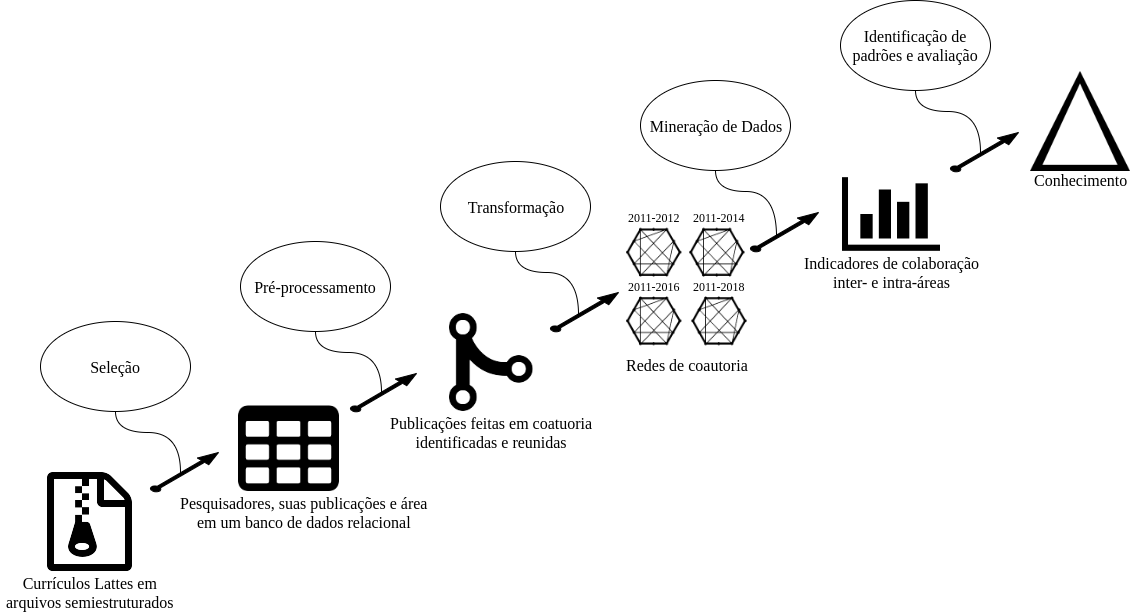
\includegraphics[scale=.3]{figuras/fayyad-diagram-graph}
  \caption{Uma visão geral dos passos adotados para o processo de descoberta de conhecimento.}
  \label{fig:processo}
\end{figure}

Este é um processo interativo e iterativo, que envolve múltiplos passos com decisões tomadas pelo pesquisador. Nas seções seguintes são discutidos os passos desse processo de descoberta de conhecimento.

\section{Seleção}

A partir de um conjunto de currículos de pesquisadores, foram extraídas informações sobre as áreas de atuação e publicações científicas, como livros, capítulos de livro, publicações em conferências e publicações em periódicos.

O \autoref{alg:selecao} apresenta o procedimento adotado, onde todos os atributos extraídos são marcados com um identificador para o currículo. Os tipos de publicações considerados neste trabalho são os livros publicados, capítulos de livro publicados, publicações completas em conferências e publicações completas em periódicos.

\begin{algorithm}
\caption{Extração de atributos do currículo do pesquisador}
\label{alg:selecao}
\begin{algorithmic}[1]

\Procedure{ExtraiaAtributos}{$id, curriculo$}
\State $A\gets \Call{SelecioneAreasDeAtuacao}{id,curriculo}$
\State $P_1\gets \Call{SelecioneLivrosPublicados}{id,curriculo}$
\State $P_2\gets \Call{SelecioneCapitulosDeLivroPublicados}{id,curriculo}$
\State $P_3\gets \Call{SelecionePublicacoesCompletasEmConferencias}{id,curriculo}$
\State $P_4\gets \Call{SelecionePublicacoesCompletasEmPeriodicos}{id,curriculo}$
\State \Return $(A,P_1,P_2,P_3,P_4)$
\EndProcedure

\end{algorithmic}
\end{algorithm}

\section{Pré-processamento}

Diversas produções científicas nessa área \cite{franceschet2011collaboration} \cite{mena2013prospecccao} \cite{reuther2006managing} descrevem casos onde uma publicação têm diversos nomes (sinônimos) e casos onde diferentes publicações possuem o mesmo nome (homônimos), cujos requerem tratamento a fim de obter um resultado mais confiável na etapa seguinte.

Neste trabalho, publicações sinônimas acontecem porque não foram cadastradas no currículo Lattes com exatamente a mesma informação, por exemplo, o mesmo título, haja vista que podem ocorrer abreviações de palavras, omissões de pontuação, ou erros de digitação.

Para amenizar este cenário foi proposto o \autoref{alg:normalizacao}, que normaliza os títulos das publicações removendo diacríticos\footnote{Um diacrítico é um sinal gráfico que se coloca sobre, sob ou através de uma letra para alterar a sua realização fonética, isto é, o seu som, ou para marcar qualquer outra característica linguística.} e elementos como tags de marcação de hipertexto, que não pertencem ao título e foram identificadas no decorrer deste trabalho.

\begin{algorithm}
\caption{Normalização do título de publicações}
\label{alg:normalizacao}
\begin{algorithmic}[1]

\Procedure{NormalizeTitulo}{titulo}
\State $titulo\gets \Call{DecodifiqueCaracteresEscapadosParaHtml}{titulo}$
\State $titulo\gets \Call{RemovaMarcacaoDeHipertexto}{titulo}$
\State $titulo\gets \Call{NormalizeParaAFormaNFKD}{titulo}$
\State $titulo\gets \Call{RemovaDiacriticosDeCaracteresASCII}{titulo}$
\State $titulo\gets \Call{NormalizeParaAFormaNFC}{titulo}$
\State \Return $titulo$
\EndProcedure

\end{algorithmic}
\end{algorithm}

Publicações homônimas são mais difíceis de ocorrer pois serão comparadas apenas publicações de um mesmo tipo referentes a um mesmo ano. Ainda, para haver o casamento entre publicações, é necessário que os títulos tenham pelo menos 3 palavras, para evitar que editoriais, por exemplo, sejam considerados uma coautoria.

Caso publicações homônimas não sejam identificadas corretamente será possível observar que a lista de coautores de um autor se dividirá em dois ou mais grupos altamente interconectados, mas sem colaborações entre grupos diferentes \cite{franceschet2011collaboration}. Ao detectar casos como este, poderá ser realizado tratamento manual.

\section{Transformação}

Usando as publicações obtidas nos currículos Lattes é possível identificar dois pesquisadores como coautores se uma mesma publicação aparece em seus currículos, e com isso construir uma rede de coautoria onde os nós são pesquisadores e os vértices a coautoria entre eles. O mesmo procedimento pode ser feito por períodos (\textit{e.g.}, biênio ou triênio), onde se obtém uma série de redes de coautoria com espaçamento temporal.

Para identificar as coautorias entre quaisquer dois autores foi proposto o \autoref{alg:coautoria}, que compara todas as publicações dentro de um mesmo ano usando o algoritmo de distância Levenshtein (\autoref{alg:levenshtein}).

\begin{algorithm}
\caption{Identificação de coautorias}
\label{alg:coautoria}
\begin{algorithmic}[1]

\Procedure{IdentificaCoautoria}{P}
\State $P^2\gets P\times{P}$
\State $C\gets \emptyset$
\ForAll{$(p_1, p_2) \in P^2$}
\If{publicações já foram comparadas}
\State \textbf{continue}
\ElsIf{publicações de anos diferentes}
\State \textbf{continue}
\ElsIf{publicações do mesmo pesquisador}
\State \textbf{continue}
\ElsIf{títulos compostos por duas palavras ou menos}
\State \textbf{continue}
\ElsIf{títulos com diferença superior a 85\% no tamanho}
\State \textbf{continue}
\ElsIf{\Call{Levenshthen}{\Call{Titulo}{$p_1$},\Call{Titulo}{$p_2$}} $<$ 0.85}
\State \textbf{continue}
\Else
\State $C\gets C\cup\{(p1, p2)\}$
\EndIf
\EndFor

\State \Return $C$
\EndProcedure

\end{algorithmic}
\end{algorithm}

\begin{algorithm}
\caption{Identificação de coautorias}
\label{alg:levenshtein}
\begin{algorithmic}[1]

\Procedure{Levenshtein}{s}
\State \Return $i$
\EndProcedure

\end{algorithmic}
\end{algorithm}

\section{Mineração de dados}

Nesta etapa serão feitos os cálculos de indicadores das redes de coautoria, onde planeja-se considerar as seguintes métricas topológicas: distância média, centralidade de grau, centralidade de proximidade, centralidade de autovetor, centralidade de contribuição, PageRank e AuthorRank\footnote{O AuthorRank é definido como uma medida que descreve as interações de um autor na rede de coautoria \cite{liu2005co}.}.

Pretendemos ainda, explorar novos arcabouços computacionais para processar todos os dados coletados.

\section{Identificação de padrões e avaliação}

Será determinada a existência de alguma correlação entre os indicadores obtidos e a análise desses indicadores para determinar se existe influência (ou impacto relativo) da Ciência da Computação em outras áreas.

Complementarmente, acontecimentos históricos que possam justificar o padrão encontrado serão buscados a fim de contextualizar a avaliação.

Diferentes conceitos de aprendizado de máquina e reconhecimento estatístico de padrões serão abordados.
